\message{ !name(document.tex)}\documentclass[openany, longbibliography,slovene,a4paper,12pt]{article}
%\documentclass[openany,slovene,a4paper,12pt]{article}
\usepackage[a4paper,inner=3.5cm,outer=2.5cm,top=2.5cm,bottom=2.5cm]{geometry}

\usepackage{braket}
\usepackage{float}
\usepackage{afterpage}
\usepackage{graphicx}
\usepackage{amssymb}

\usepackage[tbtags]{amsmath}
\usepackage[T1]{fontenc}
\graphicspath{{./slike/}{../slike_vezikel_z_robom/}{/home/jure/sola/magisterij/uporabljene_slike/}
{../eps_pdf/}}
\DeclareGraphicsExtensions{.eps,.jpeg,.png,.gif,.pdf}
\usepackage[outdir=./slike/]{epstopdf}
\epstopdfsetup{
	suffix=,
}
\usepackage[multidot]{grffile}

%\usepackage[slovene]{babel}      % slovenski delilni vzorci (!)
%\usepackage[english]{babel}
\usepackage[utf8]{inputenc}
\usepackage{makeidx}
\usepackage{enumerate}
\usepackage{caption}
\usepackage{subcaption}
\usepackage[tbtags]{mathtools}

\usepackage[section]{placeins}

\usepackage[hyphens,spaces,obeyspaces]{url}
\usepackage{breakurl}


\usepackage{ragged2e}
\edef\UrlBreaks{\do\-\UrlBreaks}

\usepackage{makeidx}
\pagestyle{headings}
\makeindex
\usepackage{fancyhdr}
\usepackage[titletoc,title]{appendix}


\usepackage[sort, numbers]{natbib}
\usepackage[pdfa]{hyperref}
\usepackage[x-1a]{pdfx}
\usepackage{pdfpages}
\usepackage{breqn}


\DeclareMathOperator{\arcsinh}{arcsinh}

\def\epsfg#1#2{\epsfig{file=#1.eps,width=#2}}
\def\legendamp#1#2{\vbox{\hsize=#1\caption{\small #2}}}

\setcounter{topnumber}{4}
\setcounter{bottomnumber}{4}
\setcounter{totalnumber}{5}
\renewcommand{\topfraction}{0.99}
\renewcommand{\bottomfraction}{0.99}
\renewcommand{\textfraction}{0.0}
\setlength{\tabcolsep}{10pt}
\renewcommand{\arraystretch}{1.5}

\def\bi#1{\hbox{\boldmath{$#1$}}}
\let\oldvec\vec
\def\vec#1{\mbox{\boldmath$#1$}}
\def\pol{{\textstyle{1\over2}}}
\def\svec#1{\mbox{{\scriptsize \boldmath$#1$}}}

\newcommand{\dif}{\mathrm{d}}
\usepackage{xparse}
\DeclareDocumentCommand{\myint}{o m o o}  
{%
	\int \IfValueT{#1}{#1} \dif #2 \IfValueT{#3}{\dif#3} \IfValueT{#4}{\dif#4}
}
\newcommand{\Alpha}{A}
\newcommand{\Beta}{B}
\newcommand{\Epsilon}{E}
\newcommand{\Kappa}{K}


\begin{document}

\message{ !name(document.tex) !offset(-3) }

\section{Introduction}
One of the most important basic problems in physics is the dynamics of many-body system. Specificaly, in quantum physics and chemistry, the dynamics of electrons and their spatial distribution determine the stability of matter. But it is not just the stability that matters. Electronic structure of materials determines many macroscopic properties like thermal and electrical conductivity, their response to electronic and magnetic field, etc.

Calculation of electronic structure has always been a challenge. It quickly became apparent that direct use of schroedinger equation is not a realistic prospect for calculation of electronic structure, except for some small molecules, as it's time complexity grows exponentially as a function of electron number. With the development of computers different numerical schemes for computation of electronic structure and optimization of molecular structure have emerged. One of them is also density functional theory (DFT from now on), which has been known for roughly 50 years. Through the years DFT has developed and today it represents one of the main tools for calculation of electronic structure especially for complex molecules and crystals.

\section{Matter description}
Non-relativistic hamiltonian describing the interaction system on nuclei and electrons can be
written as follows:
\begin{equation} \label{full_hamiltonian}
\hat H= \hat T_n + \hat  T_e + \hat  W_{n-n} + \hat W_{e-e} + \hat W_{n-e} + \hat V_{ext},
\end{equation}
where $T_n$ and $T_e$ are kinetic energies of nuclei and electrons respectively,
$W_{n-n}$, $W_{e-e}$ and $W_{e-n}$ represent  nuclei-nuclei, electron-electron
and electron-nuclei interaction terms. $V_{ext}$ represents external potential
and is strictly of multiplicative nature.  Ground state of such system is given by the solution of time independent Schr{\"o}dinger equation:
\begin{equation} \label{ham_solution}
\hat H \psi = \epsilon_0 \psi_0,
\end{equation} 
where index $0$ denotes the solution with the lowest energy. In general $\psi_0$
depends on $3N$ coordinates, where $N$ is total number of particles. This means
that complex systems with more than e.g. 10 atoms are very computationally
demanding. It is common to reduce the dimensionality of the problem by employing
Born-Oppenheimer approximation in which motion of nuclei is separated from
motion of electrons, sometimes even fixed. Thus, from now on we will restrict
ourselves to hamiltonian describing only motion of electrons:
\begin{equation} \label{electron_hamiltonian}
\hat H=  \hat  T_e  + \hat W_{e-e} + \hat W_{n-e} + \hat V_{ext}.
\end{equation}
The number of electrons $N$ for a small molecules, like water, is of the order $\sim
10$. In medium sized molecules with $\sim 50-100$ atoms, the number can grow to a few
hundred, while in large molecules, like proteins, the number can grow into
thousands and ten-thousands. As one can imagine, solving a system of coupled differential equations
with such huge number of coordinates ($3N$) is still too big problem for present
computational power. This is the reason for development of approaches which,
while still being sufficiently accurate, offer faster computational times. One
of the most used theory today is density functional theory.

\section{Density functional theory - DFT}
DFT is a method, which allows us to map many-particle problem to a
single particle problem. It effectively replaces electron wave functions with
particle density.  The core of dft lies in Kohn-Sham theorems. These two theorems
ensure that stationary many-particle systems are fully characterized by their
ground state particle density. For non-degenerate case the latter is uniquely determined
by ground state many-particle wave function, which in turn is uniquely determined by the
external potential. For a simple non-degenerate case we will prove this theorem. Let us consider hamiltonian of the form:
\begin{equation} \label{ks_hamiltonian}
\hat H = \hat T + \hat W + \hat V_{ext},
\end{equation}
where $T$ is kinetic energy, $W$ is particle interaction and $V$ is external
potential determined up to a constant. Let $V_{ext}$ be such potential that
ground state $\psi_0$ is non-degenerate. Consider now the set of all $H$ of the
form (\ref{ks_hamiltonian}), which
differ only in $V_{ext}$, with non-degenerate ground state. Since kinetic and
inter-particle interaction terms are the same for all $H$ in such set, the latter
can be represented by the set of all non-equivalent potentials:
\begin{equation}
  \begin{split}
    \mathcal{V} = \{V_{ext};\quad &\textrm{V determined up to multiplication factor and a constant;}\\
    & \textrm{$\ket{\psi_o}$ is exists and is non-degenerate}\}
    \end{split}
 \end{equation}
According to the above definition we can define the set of all corresponding
ground state-densities determined up to phase as:
\begin{equation}
  \begin{split}
    \mathcal{G} = \{\psi_0; \quad &\textrm{$\psi_0$ ground state corresponding to a potential from $V$;}\\
&\textrm{ $\psi_0\sim\psi_0e^{i\phi}$   }
    \}
    \end{split}
  \end{equation}
The map from $\mathcal{V}$ to $\mathcal{G}$ is surjective by definition. What we
would like to know is if it is also injective  (\ref{bijection}), i.e. can a single $\psi_0$ be a
ground state for two non-equivalent potentials? Suppose now that $\psi_0$ is a
ground state for two non-equivalent potentials $V_{ext}$ and $V'_{ext}$.

\begin{figure}
  \centering
  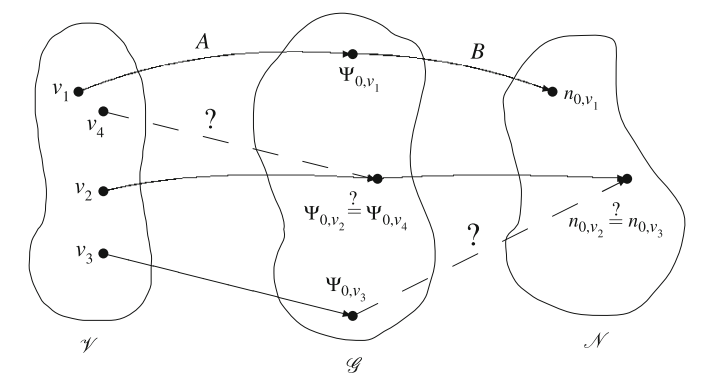
\includegraphics[width=0.55\textwidth]{bijekcija_med_v_psi_n.png}.
  \caption{Bijection between the set of potentials, their corresponding ground
    states and ground state densities. Existance of such bijection is proved by
    Kohn-Sham theorems and proves that multi-particle system is
    uniquely determined by it's ground state particle
    density~\cite{advanced_course}.}
  \label{bijection}
\end{figure}

\begin{dgroup*}
\begin{dmath}
 \hat H\ket{\psi_0} =(\hat T + \hat W + \hat V_{ext}) \ket{\psi_0}\hiderel{=}\epsilon_0\ket{\psi_0}
\end{dmath},
\begin{dmath}
 \hat H'\ket{\psi_0} =(\hat T + \hat W + \hat V'_{ext}) \ket{\psi_0}\hiderel{=}\epsilon'_0\ket{\psi_0}
\end{dmath},
\begin{dsuspend}
subtracting above equation yields:
\end{dsuspend}
\begin{dmath}
(\hat V_{ext} - \hat V'_{ext})\ket{\psi_0}=(\epsilon_0-\epsilon'_0)\ket{\psi_0}
\end{dmath}.
\begin{dsuspend}
 due to multiplicative nature of potentials, we can just divide the whole
 equation by $\ket{\psi_0}$ and obtain: 
\end{dsuspend}
\begin{dmath}
  (\hat V_{ext} - \hat V'_{ext})=(\epsilon_0-\epsilon'_0),
  \end{dmath}
\end{dgroup*}
which is contradiction, since $V_{ext}$ and $V'_{ext}$ differ for more than a
constant. Similarly one can show that two different grounds state wave functions,
corresponding to two different external potentials, cannot lead to the same
ground state densities.  To see this we compare ground state energies and rewrite
them using ground state density, which is supposed to be the same for both wavefunctions:

\begin{dgroup*}
\begin{dmath}
 \bra{\psi_o}\hat H\ket{\psi_0}=\epsilon_0 < \bra{\psi'_o}\hat H\ket{\psi'_0}=
 \bra{\psi'_o}\hat H + \hat V'_{ext} - \hat V'_{ext} \ket{\psi'_0}=\\ \epsilon'_0
 +  \bra{\psi'_o} \hat V_{ext} - \hat V'_{ext} \ket{\psi'_0}.
\end{dmath}
\begin{dsuspend}
 Rewriting this in terms of densities and taking into account equivalence of H
 and H' yields:
\end{dsuspend}
\begin{dmath}
\epsilon_0 <  \epsilon'_0 + \int (V_{ext}(\vec r)-V'_{ext}(\vec r))n(\vec r)
\dif \vec r ,
\end{dmath}
\begin{dmath}
\epsilon'_0 <  \epsilon_0 + \int (V'_{ext}(\vec r)-V_{ext}(\vec r))n(\vec r)
\dif \vec r.
\end{dmath}
\begin{dsuspend}
  Upon subtracting both equations one obtains a contradiction:
\end{dsuspend}
\begin{dmath}
  \epsilon_0 + \epsilon'_0< \epsilon_0 + \epsilon'_0,
\end{dmath}
\end{dgroup*}
which proves that for hamiltonians which yield non-degenerate ground states,
each ground state leads to a different ground state particle density. Ground
state particle densities form a set where each density corresponds to a single
wave function from $\mathcal G$:
\begin{equation}
  \mathcal N = \left\{n; \bra{\psi}\hat n \ket{\psi}, \psi \in \mathcal G \right\},
\end{equation}
where $\hat n$ is quantum mechanical particle density operator.

Extension of this simple prove to hamiltonians with degenerate ground states is possible
by replacing ground state wave functions by linear span of degenerate ground
states. Thus in degenerate case one obtains bijection between external
potential, set of linear spans, each belonging to a certain external potential
and a set of sets of ground state densities. Special treatment is necessary also
for systems containing magnetic fields, where one can separate hamiltonian into
two hamiltonians (one for each spin) of the form (\ref{ks_hamiltonian}).

Since there exists bijection between ground state wave functions and ground
state densities, one can formally rewrite ground state wave functions as functionals of ground
state particle density:
\begin{equation}
  \ket{\psi'_0} =  \ket{\psi'_0[n]},
  \end{equation}
and using above formula one can also rewrite operators in terms of ground state
density. As an example, let us rewrite ground state energy as functional of
ground state particle density:
\begin{equation} \label{hamiltonian_density}
  E[n_0] = \bra{\psi_0[n_0]}\hat H \ket{\psi_0[n_0]}.
  \end{equation}

for which one can find minimum energy principle: $E[n_0]<E[n]$ whenever n
belongs to $\mathcal N$. This an obvious consequence of wave function functional
$\ket{\psi [n]}$, which is only defined for densities which are in $\mathcal N$.
In practice this is not such a problem. The reason for this is discretization of space into
grid points. On final grid for any strictly positive particle density ($n(\vec r) > 0$),
which is compatible with Pauli principle, there exists a  potential for which the
density represents ground state density and is thus contained in $\mathcal N$.

To see that something similar also holds in general, one has to show, that
suitable wavefunctions can be constructed from a set of non-negative,
normalizable densities.
Solutions to hamiltonian of the form  (\ref{electron_hamiltonian}) are anti-symmetric $N$-particle
wave functions. Each such wave function represents a ground state corresponding
to a certain potential and for each such wavefunction on can find particle
density simpliy by applying quantum-mechanical particle density operator. But
more importantly, the conversely is also true. From each non-negative particle
density $n(\vec r)$, one can construct $N$ particle antisymmetric wavefunction
as follows:

\begin{dgroup*}
\begin{dmath} \label{phi_k}
\Phi_k(\vec r) = \sqrt { \frac{n(\vec r)}{N}} e^{i \left [\vec k \cdot \vec f (\vec r) + \phi
  (\vec r)\right]}; \quad  k \hiderel \in \mathbb{Z}, 
\end{dmath}
\begin{dsuspend}
  where $\phi(\vec r)$ is an arbitrary scalar function and $f(\vec r)$ is a
  vector field given by:
\end{dsuspend}
\begin{dmath}
  f_x(\vec r) = 2\pi \frac{ \int_{-\infty}^{x}\dif x' n(x', y,z)  } {
    \int_{-\infty}^{\infty} \dif x' n(x', y,z)    }
\end{dmath}
\begin{dmath}
  f_x(\vec r) = 2\pi \frac{ \int_{-\infty}^{\infty} \dif x'
    \int_{-\infty}^{y}\dif y' n(x', y',z)  } {
    \int_{-\infty}^{\infty} \dif x'  \int_{-\infty}^{\infty} \dif y' n(x', y' ,z)    }
\end{dmath}
\begin{dmath}
  f_x(\vec r) = 2\pi \frac{ \int_{-\infty}^{\infty} \dif x'  \int_{-\infty}^{\infty}
    \dif y'
     \int_{-\infty}^{z} \dif z' n(x', y',z')  } {
    \int_{-\infty}^{\infty} \dif x'  \int_{-\infty}^{\infty}
    \dif y'
     \int_{-\infty}^{\infty} \dif z' n(x', y', z')   }.
 \end{dmath}
 \begin{dsuspend}
Using Slater determinan one can  now construct  $N$-particle wave function from
$\phi_k({\vec r})$:
\end{dsuspend}
\begin{dmath}\label{slater_determinant}
  \Phi ({\vec r}) = \frac{1}{\sqrt{N}} \det \left(  \phi_1
    \phi_2 ...  \phi_N  \right).
  \end{dmath}
\end{dgroup*}

Above discussion tells us that minimization principle indeed holds for all
non-negative, normalizable densities, but it says nothing about definitness of
functional. For a given functional to be even defined for given particle
density, the following has to hold separately:
\begin{dgroup*}
  \begin{dmath} \label{kinetic_inequality}
    \bra{\psi}\hat T \ket{\psi} < \infty
    \end{dmath}
  \begin{dmath} \label{interaction_inequality}
    \bra{\psi}\hat W \ket{\psi} < \infty
  \end{dmath}
    \begin{dmath} \label{potential_inequality}
    \bra{\psi}\hat V \ket{\psi} < \infty.
    \end{dmath}
  \end{dgroup*}
  After deeper mathematical analysis of above equations, on can deduce that both
  $\psi$ and $n^{1/2}$ have to be from Sobolev space defined by:
  \begin{equation}
    \mathbb{H} = \left\{  f; f \in \mathbb{L}^2 \textrm{ and  } \nabla f \in \mathbb{L}^2  \right\},
    \end{equation}
  where $\mathbb{L}$ is a space of functions with finite second norm.
  Equations \ref{kinetic_inequality} and \ref{interaction_inequality} have
  imposed restrictions on permissible wavefunctions and densities. Equation
  \ref{potential_inequality} also imposes restriction on potentials. They should
  be of the form $\mathbb{L}^{3/2}+ \mathbb{L}^{\infty}$, thus every potential
  should consist of a part with a finite $\infty$-norm and a part with a
  finite ${3/2}$-norm. As it turns out, the coluomb potential satisfies all requirements.

  \subsection{Variational formualtion}
  After establishing 

  
  \section{Kohn-Sham equations}
After establishing validity of the transition from single particle wave functions
to particle density, we can now finally formulate out problem using $E[n]$. We
are looking for a minimum value of energy functional $E[n]$ with respect to particle
density n. Thus, what we have is an extremal problem: 
\begin{equation} \label{extremal_problem}
  \frac{\delta }{\delta n(\vec r)} \left[  E[n(\vec r)] - \mu \left(  \int n(\vec r) -N \right)  \right] =0.
  \end{equation}
 $E[n]$ is unfortunately still defined only formally by
 $E[n]=\bra{\psi[n]}H\ket{\psi[n]}$. To actually solve the equation
 \ref{extremal_problem}, we have to define $E[n(\vec r)]$ in terms of particle density
 $n(\vec r)$.
 
\subsection{Noninteracting system}
 First let's have a look at the hamiltonian of $N$-particle non-interacting system
 \begin{equation} \label{noninteracting_H}
   \hat H =\hat  W_k + \hat V_{ext}, 
 \end{equation}
 where $V_{ext}$ is an external potential of multiplicative nature. The solution
 to this problem can be written in the form of Slater determinant:

 \[
       \ket{\Phi_0} = \frac{1}{\sqrt{N!}}\det 
   \begin{bmatrix}
   \phi_{1}(\vec r_1, \sigma_1) & \phi_{2}(\vec r_1, \sigma_1) & \phi_{3}(\vec
   r_1, \sigma_1) & \dots & \phi_{N}(\vec r_1, \sigma_1) \\
    \phi_{1}(\vec r_2, \sigma_2) & \phi_{2}(\vec r_2, \sigma_2) & \phi_{3}(\vec
    r_2, \sigma_2) & \dots & \phi_{N}(\vec r_2, \sigma_2) \\
    \vdots & \vdots & \vdots & \ddots & \vdots \\
     \phi_{1}(\vec r_N, \sigma_N) & \phi_{2}(\vec r_N, \sigma_N) & \phi_{3}(\vec r_N, \sigma_N) & \dots & \phi_{N}(\vec r_N, \sigma_N) \\
\end{bmatrix},
\]
 which, when inserted into equation (\ref{noninteracting_H}) effectively produces
 single particle problem:
 \begin{equation}
   \left(-\frac{\hbar^2}{2m}\nabla^2 + \hat V_{ext}(\vec r)\right) \psi (\vec r) = \epsilon_i \psi(\vec r).
 \end{equation}
 Thus, using slater determinant we have effectively converted many particle
 problem with $3N$ coordiantes to a single particle problem.
 The ground state of such a system is obtained using $N/2$ lowest states and
 putting 2 electrons into each state. Calculation of kinetic energy and particle
 density for such a system is also straight forward. As we can see, using Slater
 determinant as ansatz for the solution of noninteracting hamiltonian offers
 simple expressions for ground state wavefunction, kinetic energy, density
 calculation.  

Now we would like to use similar construction to solve hamiltonian
\ref{hamiltonian_density}. Using solution ansatz in the form of Slater
determiant or some other sum of basis functions (commonly called orbitals) offers straight forward
calculation of kinetic energy and  particle density. It might be worth to point
out that dft packages usually do not use Slater determinant to construct
wavefunctions and calculate density. Using Slater determinant leads to
differentail equations for $\phi_k$ wavefunctions. Instead, they usually use
large sets of gaussian basis functions, which allow quick integral evaluation.
 

First we have to ask ourselves if it is at all possible to convert interacting
$N$ particle problem ($3N$ coordinates) to a single particle (3 coordinates)
problem. To see how this is possible consider a $N$ particle interacting system
with $n(\vec r)_{i0}$ ground state particle density. Since it represents ground
state,  this particle density belongs to $\mathcal H$. Further, using equation
(\ref{slater_determinant}) one can construct non-interacting many particle wave
function, which minimizes hamiltonian of the form (\ref{noninteracting_H})
for some potential $V_{ext}$. Thus, we see that there exists a non-interacting
system with exactly the same ground state particle density as originally
considered interacting system. The question what kind of potential to use in
place of many particle interaction operators still remains open.  

\subsection{All electron dft calculations}
All electron dft calculations are mostly used to calculate electronic structure of
 a single molecule. The molecule should not be too big, as otherwise the problem
 may become too computationally expensive. 

\subsection{Dft using pseudopotentials}
Electronic states of an atom can be divided into three categories; core states,
semi-core states and valence states. The latter are the most actively included
in formation of bonds. Valence states may be completely deformed once the atom
is put into molecules/crystals. Semi-core state are states which do not
directly contribute to bonding, but may still be polarized or spatially
deformed. Lastly, core states, are highly localized and are assumed to be
unaffected by chemical bonding. This means that there should be very little loss
of accuracy if core states are replaced by a pseudo wavefunction.
Pseudo potentials are constructs which try to
replicate effects of core electrons exerted on semi-core, valence electrons and
thus reproduce correct chemical and physical properties (bonding energy, bond
length, electron localization, magnetization,...).

Of course, pseudo potentials are constructed prior to a given calculation. Thus,
they have to constructed using some other information. As a consequence, there
exists a question of transferability. Is a potential constructed using some
reference molecule usable for another molecule. The exact answer is
not possible. Many times the only way is to try, especially when transition
elements are in question.


\section{Dft in crystals}
Crystals are periodic structures. This fact is also reflected the shape of
electronic  wave functions, which are Bloch states:
\begin{equation}
  \psi_{n, \vec k}(\vec r) = u_{n, \vec k}(\vec r)e^{i\vec k \vec r};\quad \textrm\quad u_{n,\vec k}(\vec r + \vec R) =  u_{n,\vec k}(\vec r),
\end{equation}
where $\vec R$ is a vector is Bravais lattice of a crystal in question.
Functions $u_{n,\vec k}$ depend on potential at each atomic site.
In ideal case, where core potentials are neglected,
wave functions are simple plane waves. When potential is weak and
reasonably smooth, it can be treated as perturbation. Unfortunately neither of
the two conditions is true. Core potential diverges as $r \rightarrow 0$
and as a consequence the wave functions have a cusp at the origin. For heavier
atoms core states have large gradients and can not be represented as plane waves.

The simplest solution is to expand wave functions into series of plane waves.
Computationally this is just a discrete fourier transform of a wave function.
However, because of already given reasons, the number of plane waves required
for such expansion is very large. Thus, even the sum of plane waves is not a
suitable representation of core states. For this reason, core states are
commonly replaced by pseudo potentials in crystal dft calculations. This
approach usually carries \emph{PW calculation} designation.

Although, for many
crystals this approach works well it is no good enough especially for transition elements with
partially filled d-shells and second row elements. Electron density of transition
metals and second row elements still varies widely in spite of use of
pseudopotentials. For such cases an improved approach has been developed. A new
method, called gaussian augmented plane waves or \emph{GAPW} approach. GAPW
basis sets consist of Gaussian functions and plane waves. This approach is suitable for all electron
calculations, where core states are expanded in Gaussian functions and valence
electrons in plane waves. As a consequence, all electron wave calculations are
possible for crystals avoiding pseudo potential inaccuracy issues.


%\newpage \phantomsection
\addcontentsline{toc}{section}{Literatura}
\bibliographystyle{myapsrevSLO}
\bibliography{mybib}

\end{document}
\message{ !name(document.tex) !offset(-481) }
